\documentclass[12pt]{article}

%-------------PACKAGES------------- 
\usepackage[margin=1in]{geometry} 
\usepackage{amsmath,amsthm,amssymb}
\usepackage{pgfplots}
\usepackage{float}
\usepackage{braket}
\usepackage{titling}
\usepackage{wrapfig}
\usepackage{tikz}
\usepackage{mwe}
\usepackage{enumitem}
\usepackage{mathtools}
\usepackage{scrextend}
\usepackage{listings}
\usepackage{color}
\usepackage{caption}
\usepackage{subcaption}
\usepackage{algorithm,algpseudocode}
\usetikzlibrary{shapes,arrows,chains}
\usetikzlibrary[calc]

%-------------FORMATTING-------------
\setlength{\droptitle}{-7.5em} 
\setlength{\parindent}{0pt}
\def\LW{\dimexpr.25\linewidth-.5em} 
\tikzstyle{line} = [draw, -latex']

%--------------COMMANDS--------------
\newcommand{\N}{\mathbb{N}}
\newcommand{\Z}{\mathbb{Z}}
\newcommand{\R}{\mathbb{R}}
\newcommand{\C}{\mathbb{C}}
%\renewcommand{\qedsymbol}{\filledbox}

\DeclarePairedDelimiter \abs{\lvert}{\rvert}%
\DeclarePairedDelimiter \babs{\bigg\lvert}{\bigg\rvert}%
\DeclarePairedDelimiter \norm{\lVert}{\rVert}%

%------------ENVIRONMENTS------------- 
\newenvironment{theorem}[2][]{\begin{trivlist}
		\item[{\bfseries #1}\hskip \labelsep {\bfseries #2.}]}{\end{trivlist}}
\newenvironment{lemma}[2][Lemma]{\begin{trivlist}
		\item[\hskip \labelsep {\bfseries #1}\hskip \labelsep {\bfseries #2.}]}{\end{trivlist}}
\newenvironment{exercise}[2][Exercise]{\begin{trivlist}
		\item[\hskip \labelsep {\bfseries #1}\hskip \labelsep {\bfseries #2.}]}{\end{trivlist}}
\newenvironment{reflection}[2][Reflection]{\begin{trivlist}
		\item[\hskip \labelsep {\bfseries #1}\hskip \labelsep {\bfseries #2.}]}{\end{trivlist}}
\newenvironment{proposition}[2][Proposition]{\begin{trivlist}
		\item[\hskip \labelsep {\bfseries #1}\hskip \labelsep {\bfseries #2.}]}{\end{trivlist}}
\newenvironment{corollary}[2][Corollary]{\begin{trivlist}
		\item[\hskip \labelsep {\bfseries #1}\hskip \labelsep {\bfseries #2.}]}{\end{trivlist}}
\newenvironment{definition}[2][]{\begin{trivlist}
		\item[{\bfseries #1}\hskip \labelsep {\bfseries #2.}]}{\end{trivlist}}
\theoremstyle{remark}
\newtheorem*{remark}{Remark}

%-------------CODE-STYLE------------
\definecolor{dkgreen}{rgb}{0,0.6,0}
\definecolor{gray}{rgb}{0.5,0.5,0.5}
\definecolor{mauve}{rgb}{0.58,0,0.82}
\lstset{frame=tb,
	language=C++,
	aboveskip=3mm,
	belowskip=3mm,
	showstringspaces=false,
	columns=flexible,
	basicstyle={\small\ttfamily},
	numbers=none,
	numberstyle=\tiny\color{gray},
	keywordstyle=\color{blue},
	commentstyle=\color{dkgreen},
	stringstyle=\color{mauve},
	breaklines=true,
	breakatwhitespace=true,
	tabsize=3
}

\tikzset{
	path image/.style={
		path picture={
			\node at (path picture bounding box.center) {
				\includegraphics[height=3cm]{example-image}};}},
	path tikzimage/.style={
		path picture={
			\node at (path picture bounding box.center)
			[circle, fill=blue!50, scale=2, text=yellow]{Bravo};}}
}

\lstset{
	morekeywords={end}
}

%------------------------------------ 
%---------START-OF-DOCUMENT----------
%------------------------------------
\begin{document}
	
	\title{Paper Summary}
	\author{David Miller \\ 
		CIS 5930: Social Network Mining} 
	
	\maketitle 
	
	\begin{figure}[H]{}
		\centering
		\vspace{-15pt}
		\hspace{-10pt}
		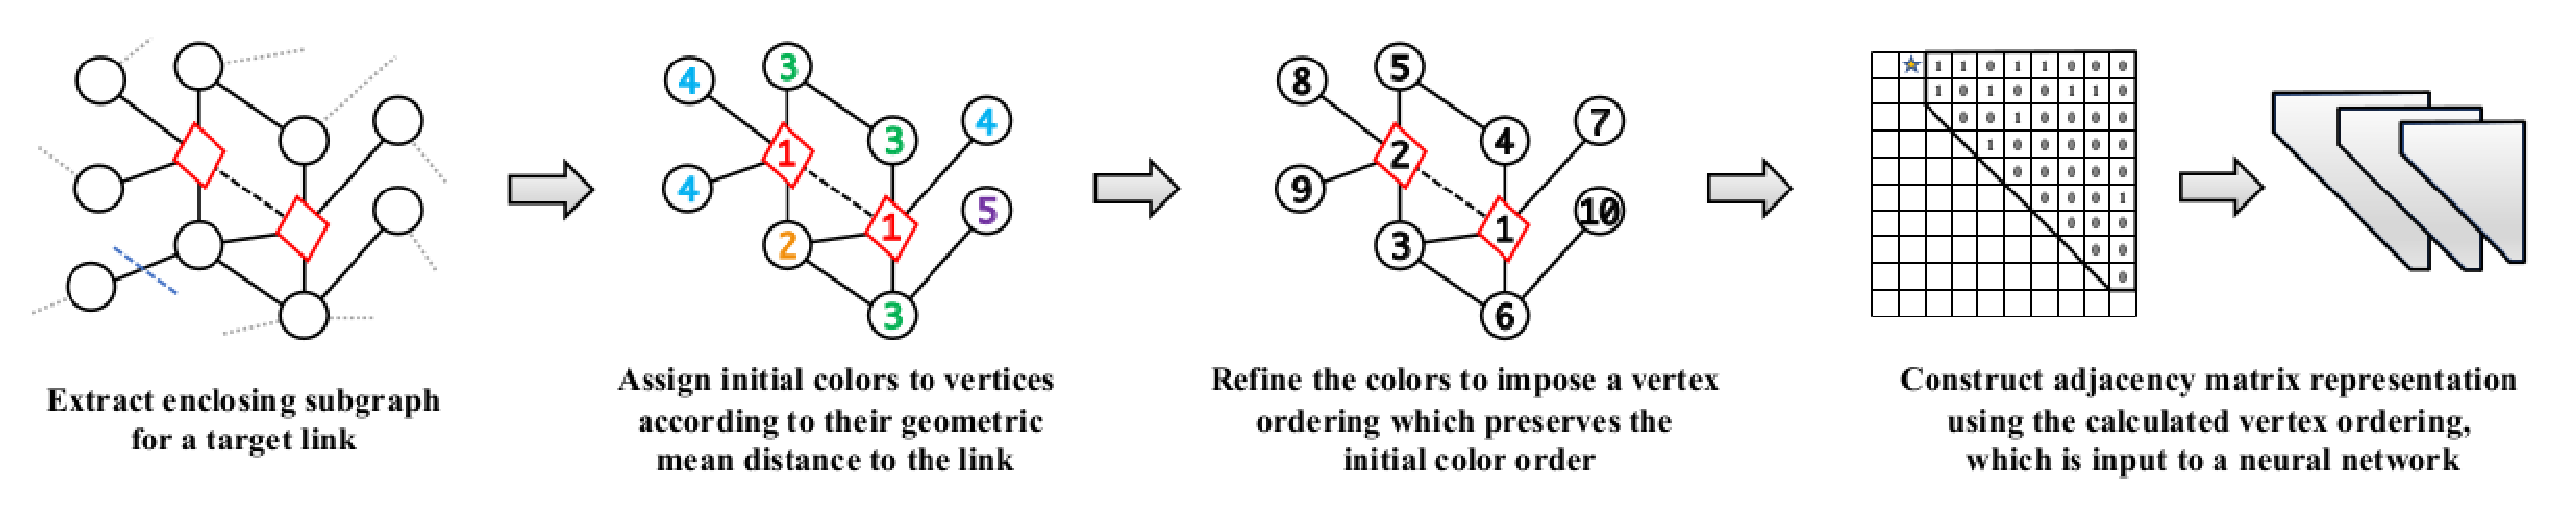
\includegraphics[height=3.5cm,width=1\textwidth]{fig1.eps}
		\caption{}
		\vspace{0pt}
	\end{figure} 
	
	The paper proposes a novel algorithm, WLNM, for link prediction. Two important concepts for link prediction are heuristics  and graphs. Heuristic methods for link prediction include first order, second order, and high order. First order methods compute based on 1-hop neighborhoods $\Gamma^1(x)$ of link vertex $x$. Second order and higher order compute via $\Gamma^2(x)$ and $\Gamma^d(x)$, respectively, for $d = 2, 3, \dots$. A network can be represented as a graph $G = (V,E)$ whose adjacency matrix $A$ will be used as input for the algorithm.  The WLNM algorithm can be summarized as follows
	\begin{enumerate}
		\item \textbf{Enclosing Subgraph Extraction :} Target link $(x,y)$ is fed as input and the algorithm iteratively builds a subgraph with vertices $(x,y)$ then $(x,y,\Gamma^1(x), \Gamma^1(y)), \dots \\ (x,y,\Gamma^1(x), \Gamma^1(y), \, \dots , \Gamma^n(x), \Gamma^n(y))$ until some threshold size $K$ is reached. 
		\item \textbf{Subgraph Pattern Encoding :} A color-order preserving algorithm is run on the subgraph. This defines structural roles (coloring) and rankings via relative positions and structural roles (ordering).
		\item \textbf{Neural Network Learning :} After the encoding step, a classifier is trained to learn complex non-linear patterns in the graph. Both positive samples ($(x,y) \in E$) and negative samples ($(x,y) \not\in E$) are used in the training process. 
	\end{enumerate}
	
	The algorithm was tested with eight datasets: USAir, NS, PB, Yeast, C.ele, Power,
	Router, and E.coli. The algorithm was tested against nine heuristic methods: common neighbors (CN), Jaccard (Jac.), Adamic-Adar (AA), resource allocation (RA),
	preferential attachment (PA), Katz, resistance distance (RD), PageRank
	(PR), and SimRank (SR). The WLNM algorithm for link prediction produced results that are superior than those it was tested against in almost every dataset. In terms of future work, I believe it should be focused on scalability. Todays market for efficient algorithms is huge, but if it can not be done via mobile computing or through personal computers, it suffers from needing time to run the algorithm and money to buy a set up that can actually run it. This algorithm has many commercially ready applications, but until it can be done with low computational cost, the only people I can see being interested in this is Amazon and Google. \\
	
	Three strengths I found with the paper are
	\begin{enumerate}
		\item The accuracy in link prediction makes it very applicable to socila networking, product recommendation, knowledge graph completion, and finding interactions between proteins. 
		\item The framework of the algorithm is based upon existing work, making it an easy to understand algorithm. This is a particularly good aspect for people who want to use the algorithm.
		\item The code is available to the public. This allows people to already use the code or improve upon it.
	\end{enumerate} 
	\vspace{0.5cm}
	
	Three weaknesses I found with the paper are
	\begin{enumerate}
		\item There was no mention of scalability. This is vital for algorithms to survive because lower execution time means cost effective and usability without warehouse scale computing. 
		\item There was not much information regarding time complexity, which leads me to believe that \, although effective, the WLNM algorithm may not be all that fast. This in turn makes it less likely to be commercially used. 
		\item There is no mention of weighted graphs. Weighted graphs are pivotal in modeling and lack of support for this could be huge negative about this algorithm.
	\end{enumerate}
	\vspace{0.5cm}
	
	Questions for the reader
	\begin{enumerate}
		\item How is the algorithm implemented for a directed network?
		\item How much data is needed to accurately train the neural network for this algorithm to produce accurate results.
	\end{enumerate}
	\vspace{0.5cm}
	
	\begin{thebibliography}{unsrt}
		\bibitem{paper}
		Muhan Zhang, Yixin Chen, \emph{Weisfeiler-Lehman Neural Machine for Link Prediction}, KDD’17, August 13-17, 2017, Halifax, NS, Canada.
	\end{thebibliography}
	
\end{document}\documentclass[12pt]{article}